\documentclass{article}
\usepackage{changepage}
\usepackage{float}
\usepackage{amsmath}
\usepackage{tikz}
\usepackage{graphicx}
\usepackage{color}
\usepackage{listings}

\definecolor{dkgreen}{rgb}{0,0.6,0}
\definecolor{gray}{rgb}{0.5,0.5,0.5}
\definecolor{mauve}{rgb}{0.58,0,0.82}

\lstset{frame=tb,
  language=Java,
  aboveskip=3mm,
  belowskip=3mm,
  showstringspaces=false,
  columns=flexible,
  basicstyle={\small\ttfamily},
  numbers=none,
  numberstyle=\tiny\color{gray},
  keywordstyle=\color{blue},
  commentstyle=\color{dkgreen},
  stringstyle=\color{mauve},
  breaklines=true,
  breakatwhitespace=true,
  tabsize=3
}
\long\def\/*#1*/{}
\begin{document}
\noindent
\begin{center}
Andreas Landgrebe
\\
Computer Science 250: Analysis of Algorithms
\\
Laboratory Assignment 3
\\
Verification of Sorting Algorithm Performance Across Datatypes
\end{center}

\newpage
\begin{center}
Part 1: Sorting Doubles
\end{center}

\begin{figure}[H]
\centering
\begin{adjustwidth}{-3.2cm}{}
\begin{tabular}{| l | l | l | l | l | l | l | l |}
\hline
Selection vs Insertion & Run 1 & Run 2 & Run 3 & Run 4 & Run 5 & Mean(Average) & Standard Deviation\\ \hline
Array Length 100 & 2.333 &1.000 & 1.206 & 1.091 & 0.900 & 1.306 & 0.52334042458041 \\ \hline
Array Length 1000 &1.008 &1.078 & 1.034 & 1.064  & 1.053 & 1.0474 & 0.024393441741583 \\ \hline
Array Length 10000 & 1.231 & 1.394 & 1.089 & 1.099 & 1.129  & 1.1884 & 0.11444404746425 \\ \hline

\end{tabular}
\caption{Results from Running Doubles of Selection vs. Insertion}
\end{adjustwidth}
\end{figure}
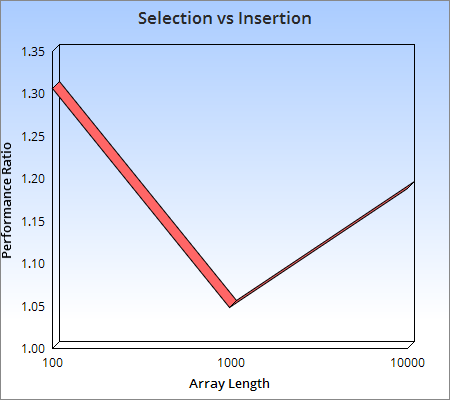
\includegraphics[scale=0.5]{Doubles1.png}
\begin{center}
Part 1: Sorting Doubles
\end{center}

\begin{figure}[H]
\centering
\begin{adjustwidth}{-3.4cm}{}
\begin{tabular}{| l | l | l | l | l | l | l | l |}
\hline
Insertion vs. Shell & Run 1 & Run 2 & Run 3 & Run 4 & Run 5 & Mean(Average) & Standard Deviation\\ \hline
Array Length 1000 & 0.098 & 0.100 & 0.099  & 0.099  & 0.101  & 0.0994 &
0.0010198039027186  \\ \hline
Array Length 10000 & 0.015 & 0.018 & 0.020 & 0.011 & 0.016  & 0.016 & 0.0030331501776206 \\ \hline
Array Length 100000 &0.002  & 0.003  & 0.003 & 0.002 & 0.002  & 0.0024 & 0.00048989794855664  \\ \hline
\end{tabular}
\caption{Results from Running Doubles of Insertion vs. Shell}
\end{adjustwidth}
\end{figure}
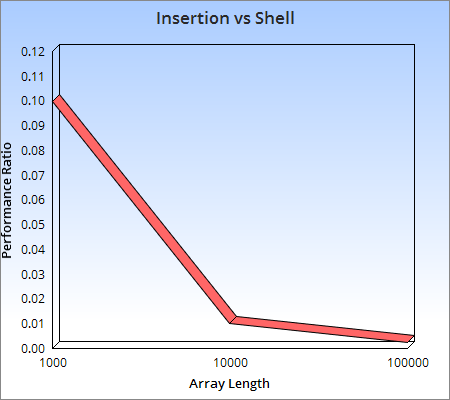
\includegraphics[scale=0.5]{Doubles2.png}
\begin{center}
Part 1: Sorting Doubles
\end{center}

\begin{figure}[H]
\centering
\begin{adjustwidth}{-3.4cm}{}
\begin{tabular}{| l | l | l | l | l | l | l | l |}
\hline
Shell Sort vs. Top-Down Merge & Run 1 & Run 2 & Run 3 & Run 4 & Run 5 & Mean(Average) & Standard Deviation\\ \hline
Array Length 10000 & 0.984 & 1.093 & 0.985 & 0.990 & 1.049 & 1.0202 & 0.04379680356331  \\ \hline
Array Length 100000 & 0.581 & 0.561 & 0.562 & 0.565 & 0.580 & 0.5698 & 0.0088408144421201 \\ \hline
Array Length 1000000 & 0.336 & 0.329 & 0.345 & 0.329 & 0.330 & 0.3338 & 0.0061773780845922  \\ \hline
\end{tabular}
\caption{Results from Running  Doubles  of Shell Sort vs. Top-Down Merge}
\end{adjustwidth}
\end{figure}
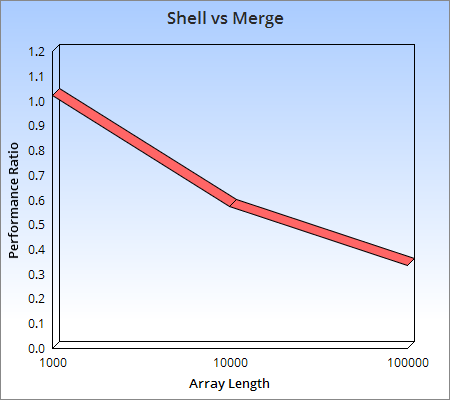
\includegraphics[scale=0.5]{Doubles3.png}




\begin{figure}[H]
\centering
\begin{adjustwidth}{-3.4cm}{}
\begin{tabular}{| l | l | l | l | l | l | l | l |}
\hline
Top Down Merge vs. Bottom Up & Run 1 & Run 2 & Run 3 & Run 4 & Run 5 & Mean(Average) & Standard Deviation\\ \hline
Array Length 10000 & 1.096 & 0.974 & 0.931 & 0.851 & 0.838 & 0.938 & 0.093678172484309 \\ \hline
Array Length 100000 & 1.009 & 1.031 & 1.010 & 1.004 & 1.000 & 1.008 & 0.010721940122944 \\ \hline
Array Length 1000000 & 1.209 & 1.220 & 1.128 & 1.122 & 1.223 & 1.1804 & 0.045513075044431  \\ \hline
\end{tabular}
\caption{Results from Running  Doubles of Top-Down Merge vs. Bottom-Up}
\end{adjustwidth}
\end{figure}

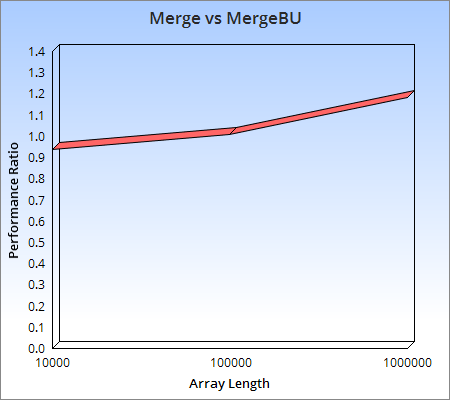
\includegraphics[scale=0.5]{Doubles4.png}

\newpage
\begin{center}
Part Two: Sorting Integers
\end{center}


\begin{figure}[H]
\centering
\begin{adjustwidth}{-3.4cm}{}
\begin{tabular}{| l | l | l | l | l | l | l | l |}
\hline
Selection vs. Insertion & Run 1 & Run 2 & Run 3 & Run 4 & Run 5 & Mean(Average) & Standard Deviation\\ \hline
Array Length 100 & 0.545 & 1.364 & 2.067 & 0.615 & 0.643 & 1.0468 & 0.59037831938512 \\ \hline
Array Length 1000 & 1.192 & 1.162 & 1.103 & 1.112 & 1.104 & 1.1346 & 0.036031097679643  \\ \hline
Array Length 10000 & 1.318 & 1.319 & 1.313 & 1.311 & 1.317  & 1.3156 &  0.0030724582991475 \\ \hline
\end{tabular}
\caption{Results from Running  Integers of Selection vs. Insertion}
\end{adjustwidth}
\end{figure}

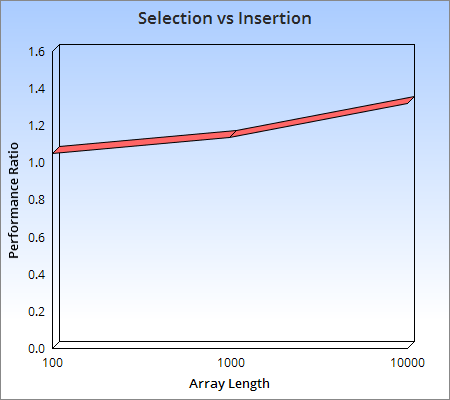
\includegraphics[scale=0.5]{Integer1.png}
\begin{figure}[H]
\centering
\begin{adjustwidth}{-3.4cm}{}
\begin{tabular}{| l | l | l | l | l | l | l | l |}
\hline
Insertion vs Shell & Run 1 & Run 2 & Run 3 & Run 4 & Run 5 & Mean(Average) & Standard Deviation\\ \hline
Array Length 1000 & 0.165 & 0.132 & 0.212 & 0.149 & 0.146 & 0.1608  &  0.027665140520156 \\ \hline
Array Length 10000 & 0.017 & 0.017 & 0.016 & 0.017 & 0.017 & 0.0168 & 0.0004  \\ \hline
Array Length 100000 & 0.003 & 0.005 & 0.003 & 0.003 & 0.002  & 0.0032 & 0.00097979589711327 \\ \hline
\end{tabular}
\caption{Results from Running  Integers of Insertion vs Shell}
\end{adjustwidth}
\end{figure}
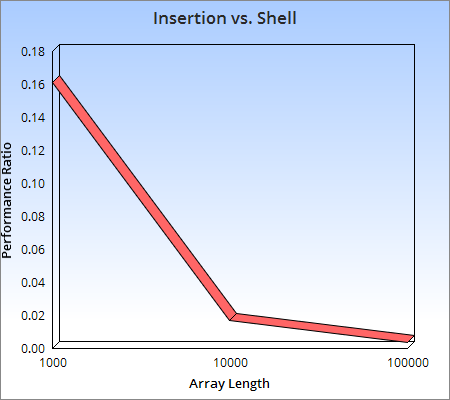
\includegraphics[scale=0.5]{Integer2.png}


\begin{figure}[H]
\centering
\begin{adjustwidth}{-3.4cm}{}
\begin{tabular}{| l | l | l | l | l | l | l | l |}
\hline
Shell vs Top-Down Merge & Run 1 & Run 2 & Run 3 & Run 4 & Run 5 & Mean(Average) & Standard Deviation\\ \hline
Array Length 10000 & 1.068 & 1.080 & 0.951 & 0.973 & 1.034 & 1.0212 & 0.051113207686468 \\ \hline
Array Length 100000 & 0.610 & 0.603 & 0.587 & 0.579  & 0.591 & 0.594 & 0.01113552872566 \\ \hline
Array Length 1000000 & 0.328 & 0.319 & 0.316 & 0.320 & 0.317 & 0.32 & 0.0042426406871193  \\ \hline
\end{tabular}
\caption{Results from Running  Integers of Shell vs. Top-Down}
\end{adjustwidth}
\end{figure}
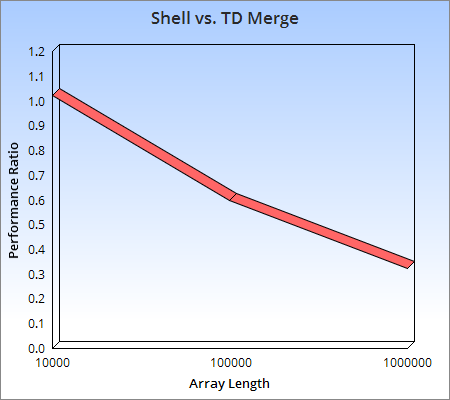
\includegraphics[scale=0.5]{Integer3.png}
\begin{figure}[H]
\centering
\begin{adjustwidth}{-3.4cm}{}
\begin{tabular}{| l | l | l | l | l | l | l | l |}
\hline
Top-Down vs Bottom-Up & Run 1 & Run 2 & Run 3 & Run 4 & Run 5 & Mean(Average) & Standard Deviation\\ \hline
Array Length 10000 & 1.139 & 1.090 & 0.963 & 0.933 & 0.880 & 1.001 & 0.097646300493157 \\ \hline
Array Length 100000 & 1.014 & 0.997 & 0.979 & 0.990 & 1.007 & 0.9974 & 0.01233855745215  \\ \hline
Array Length 1000000 & 1.171& 1.227 & 1.233 & 1.144 & 1.169 & 1.188 & 0.035010855459414 \\ \hline
\end{tabular}
\caption{Results from Running  Integers of Top-Down vs. Bottom-Up}
\end{adjustwidth}
\end{figure}
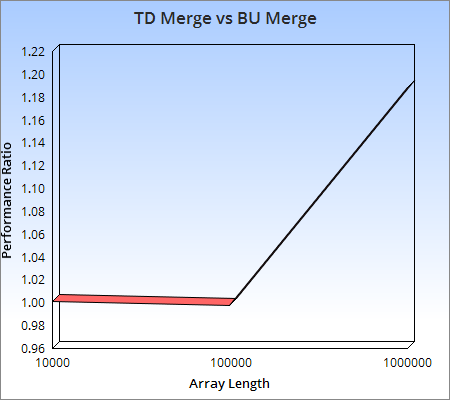
\includegraphics[scale=0.5]{Integer4.png}
\newpage
\begin{center}
Part Three: Sorting Strings
\end{center}

\begin{figure}[H]
\centering
\begin{adjustwidth}{-3.4cm}{}
\begin{tabular}{| l | l | l | l | l | l | l | l |}
\hline
Selection vs Insertion & Run 1 & Run 2 & Run 3 & Run 4 & Run 5 & Mean(Average) & Standard Deviation\\ \hline
Array Length 100 & 0.875 & 0.850 & 1.133 & 0.700 & 0.684 & 0.8484 & 0.16171406865205 \\ \hline
Array Length 1000 & 0.838 & 0.841 & 0.810 & 0.837 & 0.779 & 0.821 & 0.0237907544506741 \\ \hline
Array Length 10000 & 0.854 & 0.841 & 0.845 & 0.847 & 0.851 & 0.8476 & 0.0045431266766402 \\ \hline
\end{tabular}
\caption{Results from Running  Strings of Selection vs. Insertion}
\end{adjustwidth}
\end{figure}
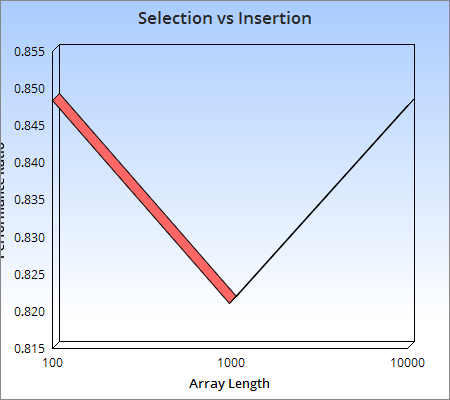
\includegraphics[scale=0.5]{String1.png}
\begin{figure}[H]
\centering
\begin{adjustwidth}{-3.4cm}{}
\begin{tabular}{| l | l | l | l | l | l | l | l |}
\hline
Insertion vs Shell & Run 1 & Run 2 & Run 3 & Run 4 & Run 5 & Mean(Average) & Standard Deviation\\ \hline
Array Length 1000 & 0.146 & 0.163 & 0.110 & 0.172 & 0.170 & 0.1522 & 0.022999130418344 \\ \hline
Array Length 10000 & 0.020 & 0.018 & 0.023 & 0.021 & 0.026 & 0.0216 & 0.0027276363393972 \\ \hline
Array Length 100000 & NA & NA & NA & NA & NA & NA & NA\\ \hline
\end{tabular}
\caption{Results from Running  Strings of Insertion vs Shell}
\end{adjustwidth}
\end{figure}
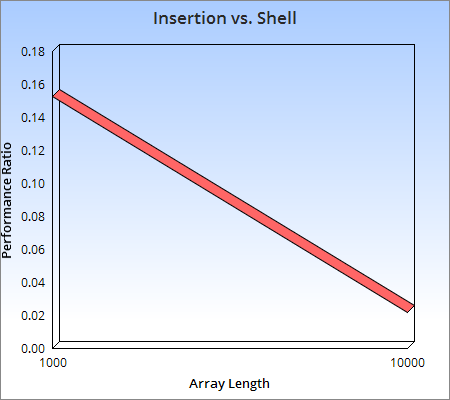
\includegraphics[scale=0.5]{String2.png}
\begin{figure}[H]
\centering
\begin{adjustwidth}{-3.4cm}{}
\begin{tabular}{| l | l | l | l | l | l | l | l |}
\hline
Shell vs Top-Down Merge & Run 1 & Run 2 & Run 3 & Run 4 & Run 5 & Mean(Average) & Standard Deviation\\ \hline
Array Length 10000 & 0.644 & 0.731 & 0.752 & 0.747 & 0.689 & 0.7126 & 0.040834299308302  \\ \hline
Array Length 100000 & NA & NA & NA & NA & NA & NA &  NA\\ \hline
Array Length 1000000 & NA & NA & NA & NA & NA & NA & NA \\ \hline
\end{tabular}
\caption{Results from Running  Strings of Shell vs Top-Down Merge}
\end{adjustwidth}
\end{figure}
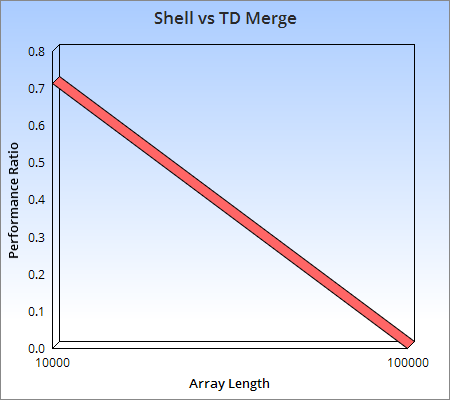
\includegraphics[scale=0.5]{String3.png}
\begin{figure}[H]
\centering
\begin{adjustwidth}{-3.4cm}{}
\begin{tabular}{| l | l | l | l | l | l | l | l |}
\hline
Top-Down vs. Bottom-Up& Run 1 & Run 2 & Run 3 & Run 4 & Run 5 & Mean(Average) & Standard Deviation\\ \hline
Array Length 10000 & 1.543 & 1.621 & 1.584 & 1.562 & 1.603 & 1.5826 & 0.027875437216302  \\ \hline
Array Length 100000 & NA & NA& NA & NA & NA & NA & NA \\ \hline
Array Length 1000000 & NA & NA & NA & NA & NA & NA & NA \\ \hline
\end{tabular}
\caption{Results from Running  Strings of Top-Down vs Bottom-Up}
\end{adjustwidth}
\end{figure}
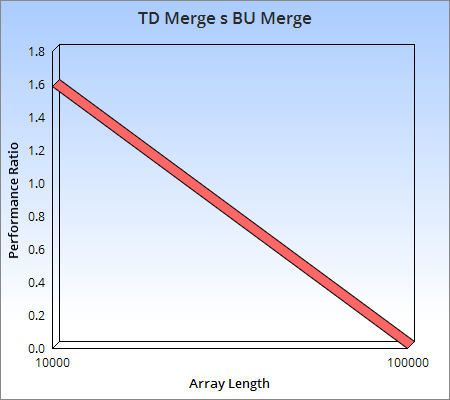
\includegraphics[scale=0.5]{String4.png}
%\begin{figure}[H]
%\centering
%\begin{adjustwidth}{-3.4cm}{}
%\begin{tabular}{| l | l | l | l | l | l | l | l |}
%\hline
%Insertion vs Shell & Run 1 & Run 2 & Run 3 & Run 4 & Run 5 & Mean(Average) & %Standard Deviation\\ \hline
%Array Length 1000 & 0.146 & 0.163 & 0.110 & 0.172 & 0.170 & 0.1522 & 0.022999130418344 \\ \hline
%Array Length 10000 & 0.020 & 0.018 & 0.023 & 0.021 & 0.026 & 0.0216 & %0.0027276363393972 \\ \hline
%Array Length 100000 & NA & NA & NA & NA & NA & NA & NA\\ \hline
%\end{tabular}
%\caption{Results from Running  Strings of Insertion vs Shell}
%\end{adjustwidth}
%\end{figure}

%\begin{figure}[H]
%\centering
%\begin{adjustwidth}{-3.4cm}{}
%\begin{tabular}{| l | l | l | l | l | l | l | l |}
%\hline
%Shell vs Top-Down Merge & Run 1 & Run 2 & Run 3 & Run 4 & Run 5 & Mean(Average) & Standard Deviation\\ \hline
%Array Length 10000 & 0.644 & 0.731 & 0.752 & 0.747 & 0.689 & 0.7126 & 0.040834299308302  \\ \hline
%Array Length 100000 & NA & NA & NA & NA & NA & NA &  NA\\ \hline
%Array Length 1000000 & NA & NA & NA & NA & NA & NA & NA \\ \hline
%\end{tabular}
%\caption{Results from Running  Strings of Shell vs Top-Down Merge}
%\end{adjustwidth}
%\end{figure}


%\begin{figure}[H]
%\centering
%\begin{adjustwidth}{-3.4cm}{}
%\begin{tabular}{| l | l | l | l | l | l | l | l |}
%\hline
%Top-Down vs. Bottom-Up & Run 1 & Run 2 & Run 3 & Run 4 & Run 5 & Mean(Average) & Standard Deviation\\ \hline
%Array Length 10000 & 1.543 & 1.621 & 1.584 & 1.562 & 1.603 & 1.5826 & 0.027875437216302  \\ \hline
%Array Length 100000 & NA & NA& NA & NA & NA & NA & NA \\ \hline
%Array Length 1000000 & NA & NA & NA & NA & NA & NA & NA \\ \hline
%\end{tabular}
%\caption{Results from Running  Strings of Top-Down vs Bottom-Up}
%\end{adjustwidth}
%\end{figure}

\newpage
\begin{center}
Part Four: Changing the Distribution
\end{center}

\begin{figure}[H]
\centering
\begin{adjustwidth}{-3.4cm}{}
\begin{tabular}{| l | l | l | l | l | l | l | l |}
\hline
Gaussian Doubles & Run 1 & Run 2 & Run 3 & Run 4 & Run 5 & Mean(Average) & Standard Deviation\\ \hline
Selection vs. Insertion  & 1.201 & 1.168 & 1.178 & 1.210 & 1.207 & 1.1928 &  0.016726027621644 \\ \hline
Insertion Sort vs Shell Sort & 0.015 & 0.015 & 0.015 & 0.016 & 0.016 & 0.0154 & 0.00048989794855664 \\ \hline
Shell Sort vs TD Merge Sort &  1.104 & 1.186 & 0.895 & 1.079 & 1.136 & 1.08 & 0.099170560147657 \\ \hline
TD Merge Sort vs BU Merge Sort & 0.898 & 0.841 & 0.940 & 0.926 & 0.986 & 0.9182 & 0.04795998331943\\ \hline
\end{tabular}
\caption{Results from Running Doubles Using Gaussian (Array length is 10000)}
\end{adjustwidth}
\end{figure}
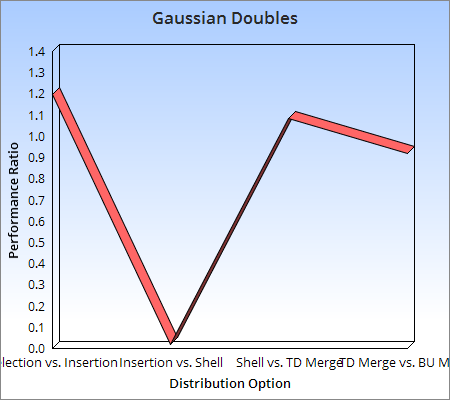
\includegraphics[scale=0.5]{GaussianDoubles.png}
\begin{figure}[H]
\centering
\begin{adjustwidth}{-3.4cm}{}
\begin{tabular}{| l | l | l | l | l | l | l | l |}
\hline
Uniform Doubles & Run 1 & Run 2 & Run 3 & Run 4 & Run 5 & Mean(Average) & Standard Deviation\\ \hline
Selection vs. Insertion  & 1.225 & 1.218 & 1.160 & 1.164 & 1.172 & 1.1878 & 0.027874002224295  \\ \hline
Insertion Sort vs Shell Sort & 0.015 & 0.015 & 0.015 & 0.016 & 0.016 & 0.0154 & 0.00048989794855664  \\ \hline
Shell Sort vs TD Merge Sort & 1.146 & 1.069 & 1.207 & 1.102 & 1.113 & 1.1274 & 0.046787177730656 \\ \hline
TD Merge Sort vs BU Merge Sort & 0.915 &0.900 & 0.825 & 0.920 & 0.929 & 0.8978 & 0.037594680474769\\ \hline
\end{tabular}
\caption{Results from Running Doubles Using Uniform  (Array length is 10000)}
\end{adjustwidth}
\end{figure}
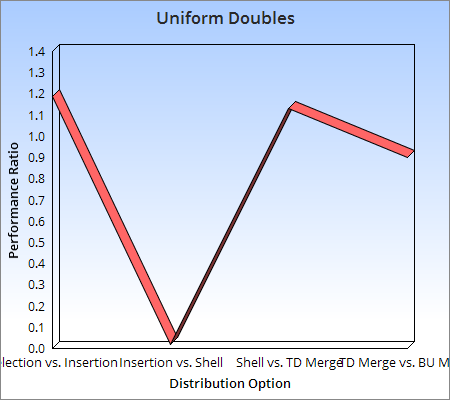
\includegraphics[scale=0.5]{UniformDoubles.png}

\begin{figure}[H]
\centering
\begin{adjustwidth}{-3.4cm}{}
\begin{tabular}{| l | l | l | l | l | l | l | l |}
\hline
Gaussian Integers & Run 1 & Run 2 & Run 3 & Run 4 & Run 5 & Mean(Average) & Standard Deviation\\ \hline
Selection vs. Insertion & 0.634 & 0.639 & 0.639 & 0.647 & 0.643 & 0.6404 & 0.004363484845854  \\ \hline
Insertion Sort vs Shell Sort & 0.009 & 0.010 & 0.010 & 0.010 & 0.009 & 0.0096 & 0.00048989794855564 \\ \hline
Shell Sort vs TD Merge Sort & 2.507 & 2.851 & 3.263 & 2.981 & 3.576 & 3.0356 &   0.36337837029741 \\ \hline
TD Merge Sort vs BU Merge Sort & 1.068 & 0.867 & 1.157 & 1.071 & 1.368 & 1.1062 & 0.16188563864655 \\ \hline
\end{tabular}
\caption{Results from Running Integers Using Gaussian (Array length is 10000)}
\end{adjustwidth}
\end{figure}

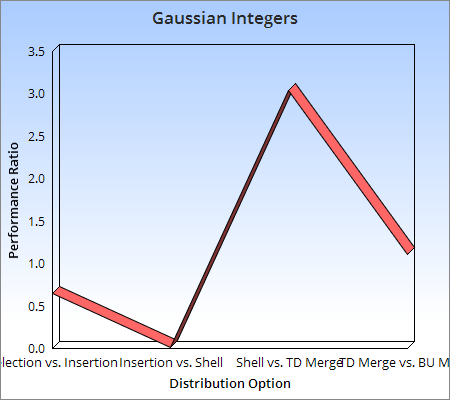
\includegraphics[scale=0.5]{GaussianIntegers.png}

\begin{figure}[H]
\centering
\begin{adjustwidth}{-3.4cm}{}
\begin{tabular}{| l | l | l | l | l | l | l | l |}
\hline
Uniform Integers & Run 1 & Run 2 & Run 3 & Run 4 & Run 5 & Mean(Average) & Standard Deviation\\ \hline
Selection vs. Insertion & 1.452 & 1.523 & 1.289 & 1.329 & 1.348 & 1.3882 & 0.08625868072258 \\ \hline
Insertion Sort vs Shell Sort & 0.021 & 0.013 & 0.019 & 0.031 & 0.026 & 0.022 &  0.0061318838867024 \\ \hline
Shell Sort vs TD Merge Sort & 1.022 & 1.170 & 0.943 & 0.814 & 1.272 & 1.0442 & 0.16213870605133\\ \hline
TD Merge Sort vs BU Merge Sort & 0.607 & 0.808 & 1.038 & 0.810 & 0.986 & 0.8498 & 0.15248134312105\\ \hline
\end{tabular}
\caption{Results from Running Integers Using Uniform (Array length is 10000)}
\end{adjustwidth}
\end{figure}
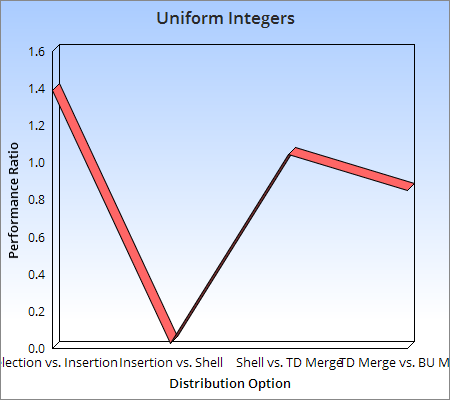
\includegraphics[scale=0.5]{UniformIntegers.png}


\begin{figure}[H]
\centering
\begin{adjustwidth}{-3.4cm}{}
\begin{tabular}{| l | l | l | l | l | l | l | l |}
\hline
Gaussian Strings & Run 1 & Run 2 & Run 3 & Run 4 & Run 5 & Mean(Average) & Standard Deviation\\ \hline
Selection vs. Insertion & 0.578 & 0.512 & 0.529 & 0.489 & 0.6603 & 0.5422 & 0.042177719236583\\ \hline
Insertion Sort vs Shell Sort & 0.019 & 0.022 & 0.021 & 0.017 & 0.018 & 0.0194 & 0.0018547236990991 \\ \hline
Shell Sort vs TD Merge Sort & 0.715 & 0.675 & 0.699 & 0.775 & 0.721 & 0.717 & 0.033081717005017\\ \hline
TD Merge Sort vs BU Merge Sort & 0.935 & 0.869 & 0.822 & 0.793 & 0.972 & 0.8782 & 0.067121978516727\\ \hline
\end{tabular}
\caption{Results from Running Strings Using Gaussian (Array length is 10000)}
\end{adjustwidth}
\end{figure}
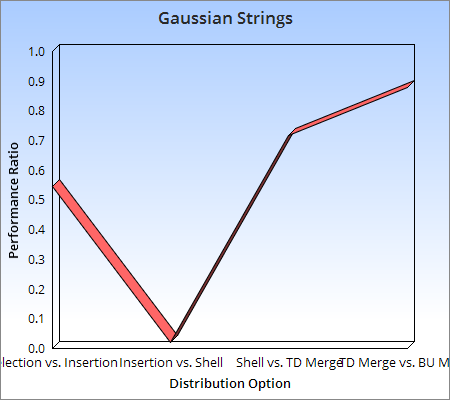
\includegraphics[scale=0.5]{GaussianStrings.png}

\begin{figure}[H]
\centering
\begin{adjustwidth}{-3.4cm}{}
\begin{tabular}{| l | l | l | l | l | l | l | l |}
\hline
Uniform Strings & Run 1 & Run 2 & Run 3 & Run 4 & Run 5 & Mean(Average) & Standard Deviation\\ \hline
Selection vs. Insertion & 0.919 & 0.827 & 0.799 & 0.948 & 0.914 & 0.8814 & 0.057725557598\\ \hline
Insertion Sort vs Shell Sort & 0.017 & 0.019 & 0.026 & 0.015 & 0.017 & 0.0188 & 0.0038157568056678 \\ \hline
Shell Sort vs TD Merge Sort & 0.676 & 0.592 & 0.661 & 0.721 & 0.612 & 0.6663266 & 0.041440347488891\\ \hline
TD Merge Sort vs BU Merge Sort & 1.283 & 1.197 & 1.321 & 1.274 & 1.289 & 1.2728 & 0.041077487751809\\ \hline
\end{tabular}
\caption{Results from Running Strings Using Uniform (Array length is 10000)}
\end{adjustwidth}
\end{figure}
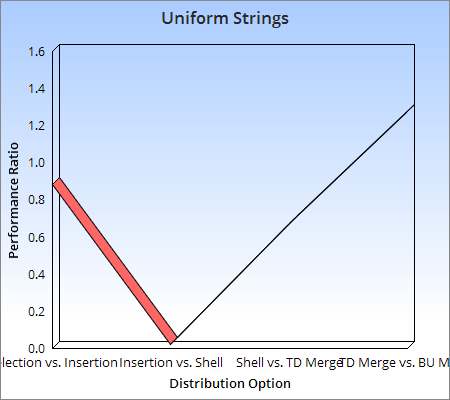
\includegraphics[scale=0.5]{UniformStrings.png}





\newpage

\begin{center}
Part Five: While You Have Some Downtime
\end{center}
\begin{enumerate}
\item Trace How:
\begin{enumerate}
\item The Selection Sort algorithm will sort the array SELECTIONSORT\\
Here are the steps for the selection sort algorithm:
\\
SELECTIONSORT\\
SELE\textbf{C}TIONSORT\\
CS\textbf{E}LETIONSORT\\
CESL\textbf{E}TIONSORT\\
CEESLT\textbf{I}ONSORT\\
CEEIS\textbf{L}TONSORT\\
CEEILSTO\textbf{N}SORT\\
CEEILNST\textbf{O}SORT\\
CEEILNOSTS\textbf{O}RT\\
CEEILNOOSTS\textbf{R}T\\
CEEILNOOR\textbf{S}TST\\
CEEILNOORST\textbf{S}T\\
CEEILNOORSS\textbf{T}T\\
CEEILNOORSST\textbf{T}\\
CEILLNOORSSTT\\

\item The Insertion Sort algorithm will soft the array INSERTIONSORT
\\Here are the steps for the insertion sort algorithm
\\
INSERTIONSORT\\
\textbf{I}NSERTIONSORT\\
I\textbf{N}SERTIONSORT\\
\textbf{S}INSERTIONSORT\\
\textbf{E}INRTIONSORT\\
EIN\textbf{R}STIONSORT\\
EINR\textbf{S}TIONSORT\\
EINRS\textbf{T}IONSORT\\
EI\textbf{I}NRSTONSORT\\
EIIN\textbf{O}RSTNSORT\\
EIIN\textbf{N}ORST\\
EIINN\textbf{O}RST\\
EIINNO\textbf{R}ST\\
EIINNOR\textbf{S}T\\
EIINNORS\textbf{T}\\
EIINNORST\\
\item The Shell Sort algorithm will sort the array SHELLSORTISSOMUCHFUNYOUGUYS
\\
The shell sort is creating partially sorted array that will be later be efficiently sorted by Insertion Sort.
\\

\item The Top-Down Mergesoft algorithm will sort the array ISNTDATACOLLECTIONFUN
\\
The merge sort will split an array into two halves, sort them,. and then merge then back into a single sorted array.
\end{enumerate}
\item Which sorting algorithm (Selection or Insertion) will run the fastest on an array where all keys are equal? Why?
\\
Insertion will run the fastest on an array because selection will always run the same amount of time since it has to iterate through the entire array and if the keys of an array is all equal, then Insertion will take a shortest amount of time to check each index in the array.
\item Which sorting algorithm (Selection or Insertion) will run the fastest on an array that is in reverse order? Why?
Selection will run quickest when the array is in reverse order since it takes a long amount of time for insertion to switch the items in the indexes and selection sort will always run the same amount of time and insertion will have cases.
\item What is the best case input Shell Sort? Why?
\\
The best case input shell sort depends on input because it depends on how big the input is going to be since it is making smaller array to later be turned into an insertion way to sort an array. 
\item (This question best answered after all tests runs are complete.) Did you notice any substantial performance differences between runs of Doubles, Integers, and Strings? What about between uniformly distributed and Gaussian-distributed values? Did you think (before experimentation) that you would see any change?
\\
I noticed that strings took the longest amount of time to perform tests since it was the biggest data structure to go through.
I also noticed that Shell ran quicker using the gaussian compared to the uniform way.  I think that I would not see any other change.
\end{enumerate}
\end{document}